%%%%%%%%%%%%%%%%%%%%%%%%%%%%%%%%%%%%%%%%%
% Thin Sectioned Essay
% LaTeX Template
% Version 1.0 (3/8/13)
%
% This template has been downloaded from:
% http://www.LaTeXTemplates.com
%
% Original Author:
% Nicolas Diaz (nsdiaz@uc.cl) with extensive modifications by:
% Vel (vel@latextemplates.com)
%
% License:
% CC BY-NC-SA 3.0 (http://creativecommons.org/licenses/by-nc-sa/3.0/)
%
%%%%%%%%%%%%%%%%%%%%%%%%%%%%%%%%%%%%%%%%%

%----------------------------------------------------------------------------------------
%	PACKAGES AND OTHER DOCUMENT CONFIGURATIONS
%----------------------------------------------------------------------------------------

\documentclass[a4paper, 10pt]{article} % Font size (can be 10pt, 11pt or 12pt) and paper size (remove a4paper for US letter paper)

\usepackage[protrusion=true,expansion=true]{microtype} % Better typography
\usepackage{graphicx} % Required for including pictures
\usepackage{wrapfig} % Allows in-line images
\usepackage{hyperref}

\usepackage[utf8]{inputenc}
\usepackage[T1]{fontenc}

\usepackage{mathpazo} % Use the Palatino font
\usepackage[T1]{fontenc} % Required for accented characters
\linespread{1} % Change line spacing here, Palatino benefits from a slight increase by default


\usepackage[top=1in, bottom=1.25in, left=1.25in, right=1.25in]{geometry}

\makeatletter
\renewcommand\@biblabel[1]{\textbf{#1.}} % Change the square brackets for each bibliography item from '[1]' to '1.'
\renewcommand{\@listI}{\itemsep=0pt} % Reduce the space between items in the itemize and enumerate environments and the bibliography

\renewcommand{\maketitle}{ % Customize the title - do not edit title and author name here, see the TITLE block below
\begin{flushright} % Right align
{\LARGE\@title} % Increase the font size of the title

\vspace{50pt} % Some vertical space between the title and author name

{\large\@author} % Author name
\\\@date % Date

\vspace{40pt} % Some vertical space between the author block and abstract
\end{flushright}
}

%----------------------------------------------------------------------------------------
%	TITLE
%----------------------------------------------------------------------------------------

\title{Sujet de stage Master ATIAM 2015-2016\\ % Title
\textbf{Apprentissage d'un espace de représentation adapté aux partitions musicales}} % Subtitle

\author{\textsc{Léopold Crestel} % Author
\\{\textit{IRCAM}}} % Institution

\date{15 Janvier 2016} % Date

%----------------------------------------------------------------------------------------

\begin{document}

\maketitle % Print the title section

%----------------------------------------------------------------------------------------
%	ABSTRACT AND KEYWORDS
%----------------------------------------------------------------------------------------

\hspace*{3,6mm}\textit{Keywords:} \textit{Deep learning}, \textit{Representation learning}, \textit{embedding space}, \textit{Music generation}

\vspace{30pt} % Some vertical space between the abstract and first section

%----------------------------------------------------------------------------------------
%	ESSAY BODY
%----------------------------------------------------------------------------------------

\section*{Contexte}

Depuis 2015, l'Institut de Recherche et Coordination Acoustique/Musique (\href{http://www.ircam.fr/}{IRCAM}) est engagé au côté de la Schulich School of Music de l'université McGill à Montréal (\href{http://www.mcgill.ca/music/}{SSM}) et de la Haute École de Musique de Genève	(\href{http://www.hesge.ch/hem/}{HEM}) dans un projet de recherche dont le but est de construire une théorie moderne de l'orchestration musicale. L'orchestration musicale peut se définir de manière générale comme l'art d'écrire des partitions musicales pour plusieurs instruments. Un aspect essentiel de l'écriture orchestrale est la manipulation des mélanges instrumentaux afin de produire différents timbres. Contrairement à l'harmonie ou  le contrepoint, il n'existe pas de théorie de l'écriture timbrale et l'enseignement de cette discipline se fait essentiellement de manière empirique à travers l'étude d'œuvres déjà écrites par des compositeurs et qui font office de "références" \cite{koechli_orch}. Cette absence de formalisme peut s'expliquer par la présence de deux obstacles : la vaste combinatoire qu'offre les mélanges d'instruments au sein d'un orchestre symphonique implique un temps d'exploration de l'espace des possibles déraisonnable pour un être humain. A cela s'ajoute notre incapacité à prédire le timbre résultant d'un mélange d'instruments. Les phénomènes non linéaires impliqués rendent difficile une caractérisation mathématique simple du timbre à partir du signal audio \cite{peeters2011timbre}. Si le cerveau humain peine à appréhender un espace de dimension aussi élevé, l'outil informatique peut en faciliter l'exploration. Parmi les nombreux objectifs de cet ambitieux projet, l'un d'eux est de réaliser une intelligence artificielle capable de générer des séquences musicales orchestrales. 
%Ce projet fait l'objet d'une thèse depuis Septembre 2015 encadrée par Philippe Esling et menée par Léopold Crestel.

Les récentes avancées dans le domaine de l'apprentissage automatique laissent entrevoir des résultats prometteurs. Un modèle ancien appelé réseaux de neurones artificiels a connu un regain d'intérêt certain depuis l'avènement en 2006 d'une nouvelle méthode d'entrainement : le \textit{Deep Learning} \cite{Hinton:2006:FLA:1161603.1161605}. 
Aujourd'hui composé de toute un famille de modèles, les réseaux de neurones artificiels (\textit{ANN} pour \textit{Artificial Neural Network}) reposent sur une analogie avec le fonctionnement du cerveaux : des unités de calcul appelées neurones implémentent une fonction non-linéaire simple. Chaque neurone reçoit en entrée un flux de donné, applique la fonction qu'il représente en envoie le résultat de son calcul à d'autres neurones. Les neurones sont organisés en couches successives que l'on peut représenter par un graphe. Chaque neurone d'une couche $l$ reçoit en entrée la sortie des neurones de la couche $l-1$.
Initialement développés dans le domaine de la vision informatique, les \textit{ANN} constituent aujourd'hui l'état de l'art en reconnaissance d'objets. Depuis peu c'est également le cas en traitement du langage naturel (\textit{Natural Langage Processing}, \textit{NLP}). Peu de travaux ont été effectués en génération automatique de musique (on citera tout de même \cite{boulanger2012modeling,DBLP:journals/corr/LiuR14a}), mais les nombreuses analogies avec les deux domaines précédemment cités incitent une investigation poussée de ces modèles.

Une étape cruciale dans la construction d'un tel modèle est de trouver une représentation adaptée des données que l'on manipule. En informatique musicale on oppose souvent données symboliques (\textit{e.g.} partition MIDI) et données audio (\textit{e.g.} forme d'onde issues d'un enregistrement). Cette étape de pré-traitement des données à pour but de transformer des données bruts  (captées par un microphone, écrites au format MIDI...) en données exploitables par un réseaux de neurones. Au-delà d'un simple import de données, une régularisation statistique est souvent nécessaire.

\section{Sujet de stage}
\begin{figure}
\begin{center}
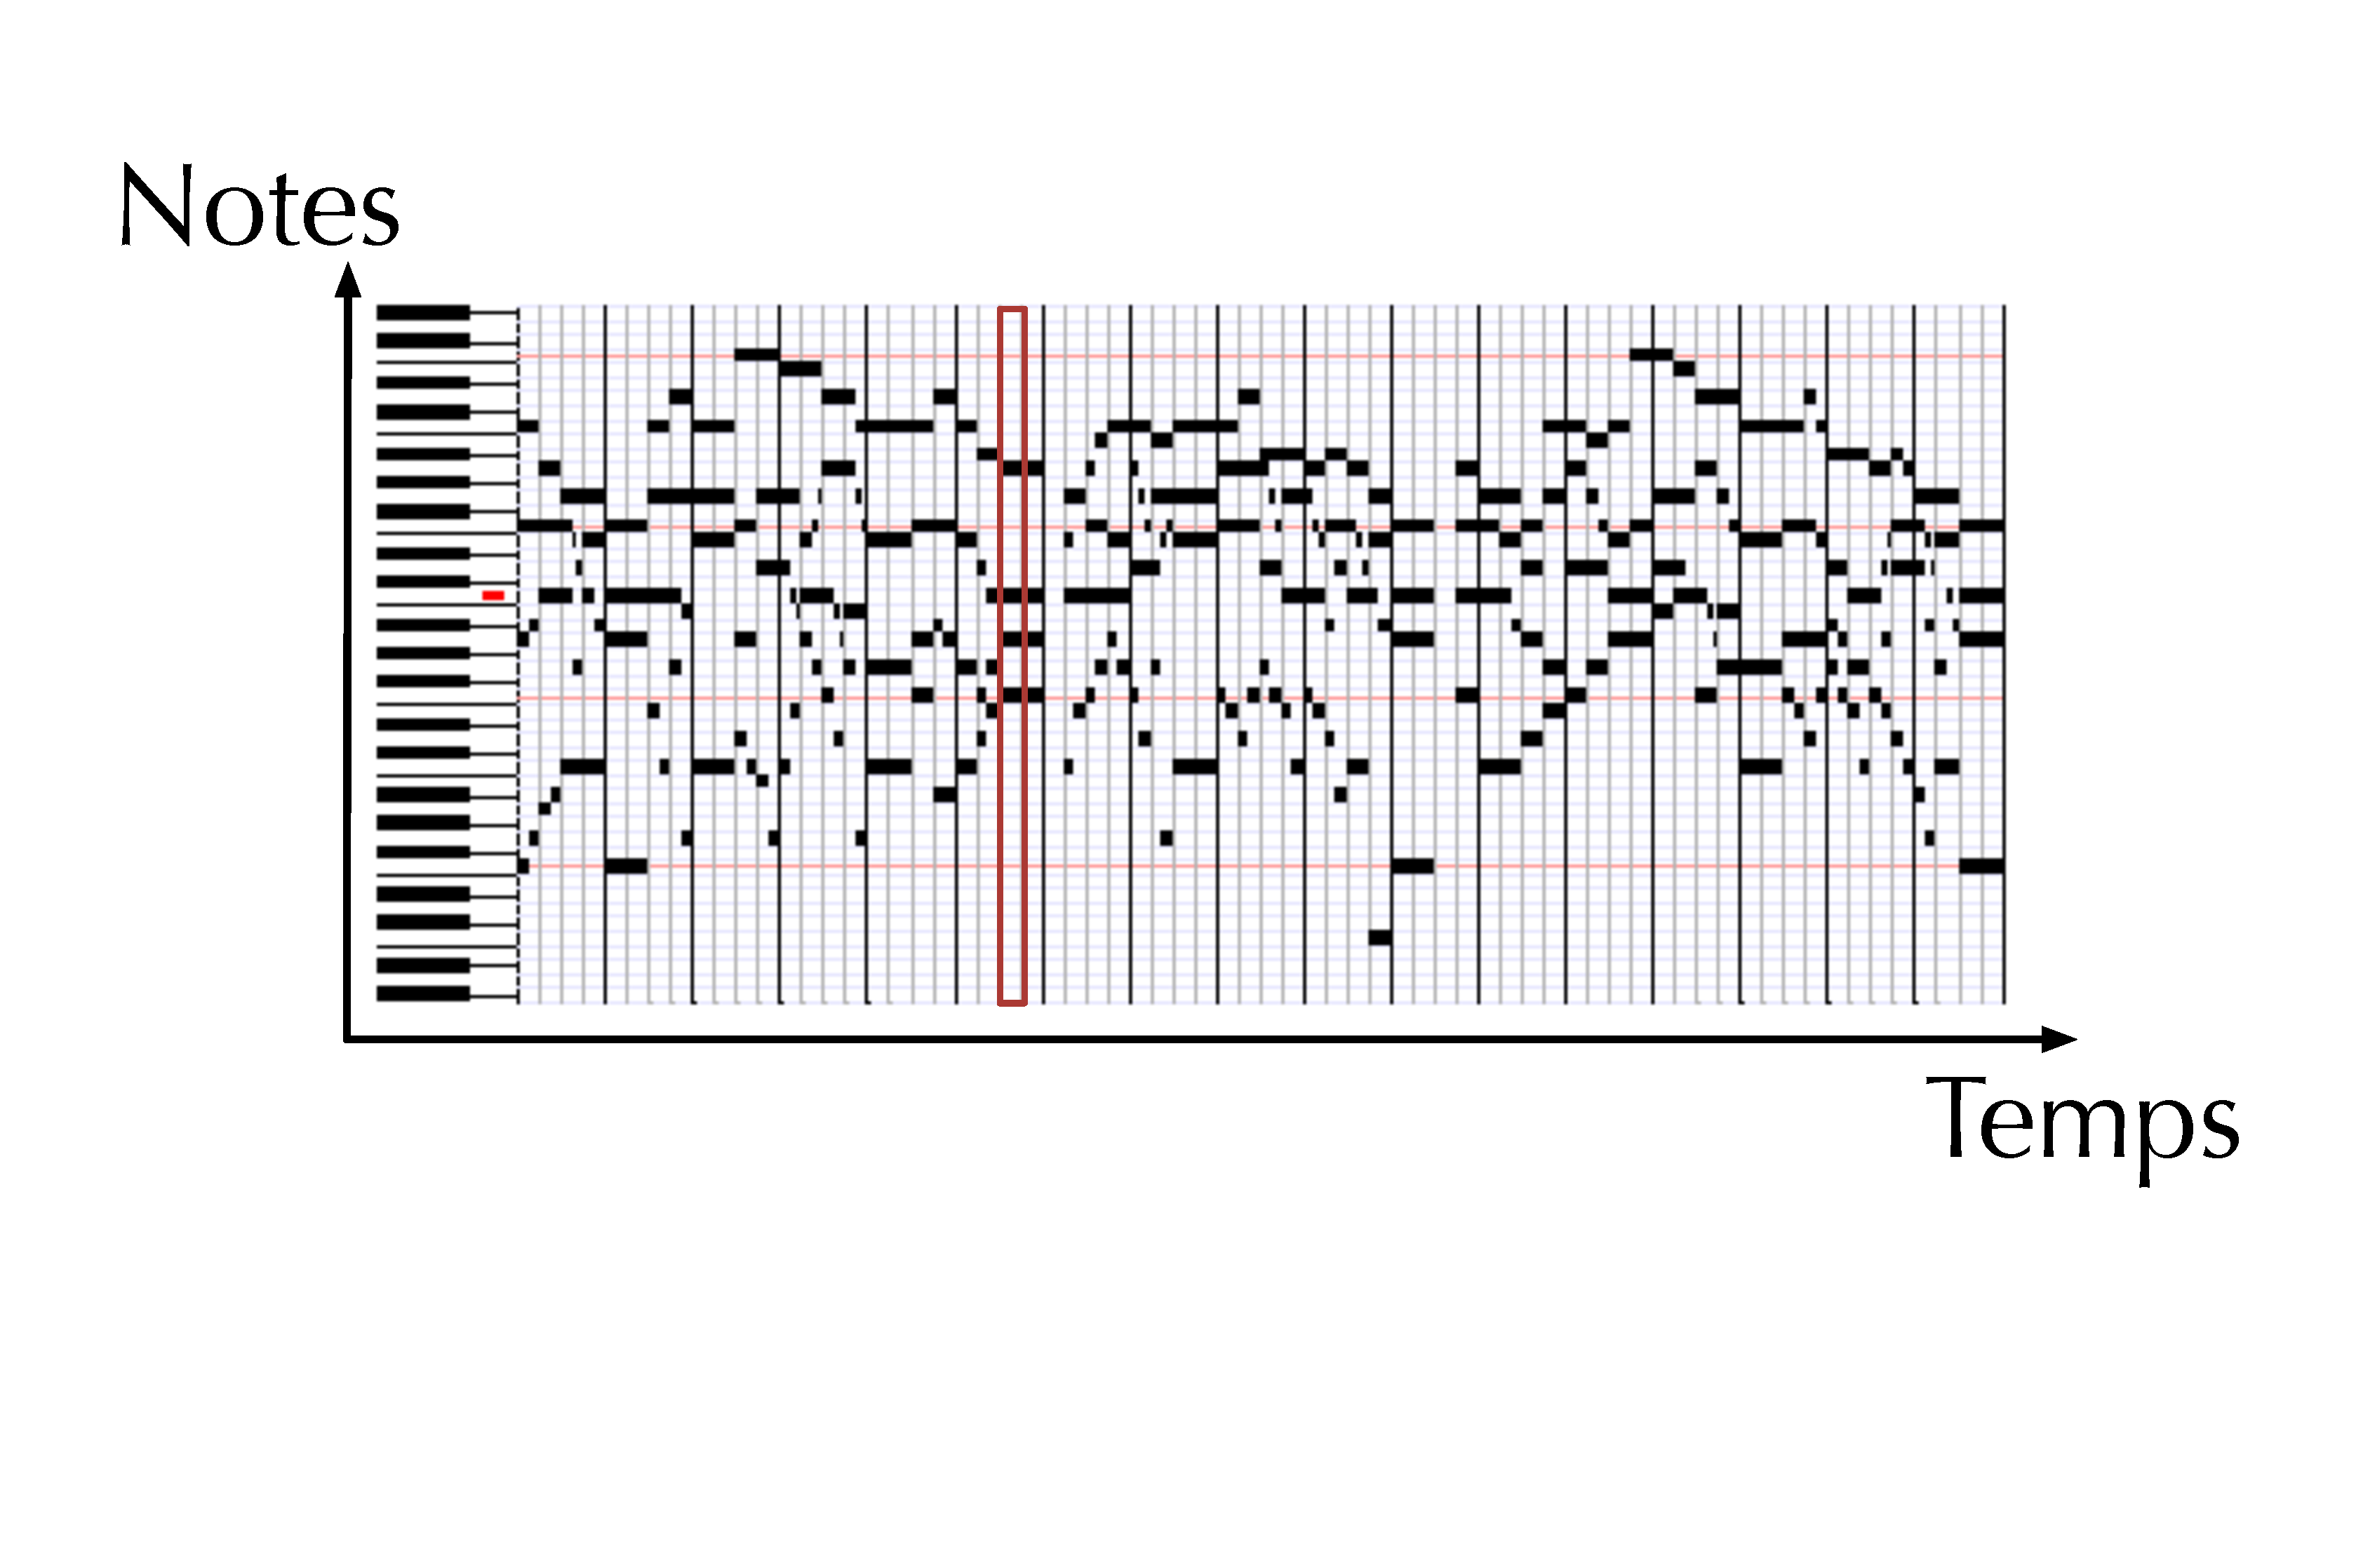
\includegraphics[scale=0.3]{../pr.pdf}
\end{center}
\label{fig:pr}
\caption{Représentation en pianoroll. Le temps est discrétisé selon une valeur symbolique de référence (typiquement une fraction de la noire) et les fréquences sont également discrétisées selon le tempérament égal en vigueur dans la musique classique occidentale. Le pianoroll est une matrice $P$ binaire dont la valeur $P(n,t)$ est égale à 1 si la note $n$ est jouée à l'instant $t$ et à 0 sinon.}
\end{figure}

Les données symboliques sont habituellement représentées à l'aide d'une structure appelée pianoroll \ref{fig:pianoroll}. La série temporelle des colonnes du pianoroll, peut être utilisée comme donnée d'entrée pour un réseau de neurone. Cette représentation "naïve" induit des vecteurs binaires parcimonieux peu adaptés aux \textit{ANN}. Le même problème survient en \textit{NLP} : chaque mot est encodé par une unique unité dans un vecteur de la taille du de l'ensemble du dictionnaire que l'on considère (\textit{one-hot encoding}). Une solution (appelée \textit{word embedding} \cite{mikolov2013efficient}) consiste à projeter ces vecteurs dans un nouvel espace de dimensionalité moins grande et à valeur réelles. Cet espace est construit automatiquement en tentant de trouver la représentation la mieux adaptée à une prédiction linéaire d'un mot en fonction de son contexte.

Cette méthode ne peut être utilisée telle quelle sur des données de musique symbolique puisque l'encodage de départ n'est pas le même (il n'y a pas qu'un valeur égale à 1). Le but du stage est d'adapter les techniques de \textit{word-embedding} au contexte musical en proposant une méthode pour trouver l'espace de plongement le mieux adapté à la génération automatique de musique. Cette représentation pourra ensuite être reliée aux travaux déjà effectués au sein de l'équipe en l'utilisant comme entrée des architectures développées. Idéalement, une rapide étude des propriétés de la représentation trouvée sera menée, afin de déterminer si elle exhibe, comme c'est le cas en \textit{NLP}, des propriétés "sémantiques" intéressantes (en musique, propriétés de translation, enchaînements harmoniques...).

Les étapes prévues pour le stage peuvent être résumées ainsi :
\begin{enumerate}
\item lecture des articles de référence de \textit{word-embedding}
\item réflexion sur les moyens d'étendre ces méthodes aux données musicales symbolique. On se posera notamment la question de la fonction d'objectif à utiliser pour construire l'espace de plongement.
\item implémenter la méthode qui semble la mieux adaptée
\item explorer les propriétés géométriques simples de cette représentations (homothéties, translations)
\end{enumerate}

%----------------------------------------------------------------------------------------
%	BIBLIOGRAPHY
%----------------------------------------------------------------------------------------

\bibliographystyle{unsrt}
\bibliography{../biblio}

%----------------------------------------------------------------------------------------

\end{document}